\documentclass[aspectratio=169,xcolor=dvipsnames]{beamer}

\usepackage{theme/beamerthemeSimpleDarkBlue}

\usepackage[utf8]{vietnam}
\usepackage{amsmath,amssymb,mathtools}
\usepackage{booktabs}
\usepackage{graphicx}
\usepackage{tikz}
\usetikzlibrary{positioning,arrows.meta,calc}

\graphicspath{{img/}{img/deep_learning/}}

\newcommand{\R}{\mathbb{R}}
\newcommand{\cp}[1]{[\![#1]\!]}
\newcommand{\had}{\ast}

% --- TikZ helpers for drawing tensors ---
\newcommand{\tfgCellW}{0.40}
\newcommand{\tfgCellH}{0.40}
\newcommand{\drawtfgface}[7]{% rows, cols, x, y, fill, draw, dashed(0/1)
  \pgfmathsetmacro{\tfgW}{#2*\tfgCellW}%
  \pgfmathsetmacro{\tfgH}{#1*\tfgCellH}%
  \draw[line width=0.55pt, fill=#5, draw=#6, rounded corners=2.0pt]
    (#3,#4) rectangle (#3+\tfgW,#4-\tfgH);
  \pgfmathtruncatemacro{\tfgRows}{#1}%
  \ifnum\tfgRows>1
    \foreach \i in {1,...,\numexpr\tfgRows-1\relax} {%
      \ifnum#7=1
        \draw[line width=0.4pt, dashed, #6!55] (#3,#4-\i*\tfgCellH) -- (#3+\tfgW,#4-\i*\tfgCellH);
      \else
        \draw[line width=0.4pt, #6!55] (#3,#4-\i*\tfgCellH) -- (#3+\tfgW,#4-\i*\tfgCellH);
      \fi
    }%
  \fi
  \pgfmathtruncatemacro{\tfgCols}{#2}%
  \ifnum\tfgCols>1
    \foreach \j in {1,...,\numexpr\tfgCols-1\relax} {%
      \ifnum#7=1
        \draw[line width=0.4pt, dashed, #6!55] (#3+\j*\tfgCellW,#4) -- (#3+\j*\tfgCellW,#4-\tfgH);
      \else
        \draw[line width=0.4pt, #6!55] (#3+\j*\tfgCellW,#4) -- (#3+\j*\tfgCellW,#4-\tfgH);
      \fi
    }%
  \fi
}
\newcommand{\drawtfgvec}[5]{% len, x, ytop, fill, draw
  \drawtfgface{#1}{1}{#2}{#3}{#4}{#5}{0}%
}
\newcommand{\drawtfgveccy}[5]{% len, x, ycenter, fill, draw
  \pgfmathsetmacro{\tfgTop}{#3+0.5*#1*\tfgCellH}%
  \drawtfgface{#1}{1}{#2}{\tfgTop}{#4}{#5}{0}%
}
\newcommand{\drawtfgtensor}[7]{% I, J, K, x, y, fill, draw
  \def\tfgOx{-0.18}\def\tfgOy{0.16}%
  \pgfmathsetmacro{\tfgW}{#2*\tfgCellW}%
  \pgfmathsetmacro{\tfgH}{#1*\tfgCellH}%
  \pgfmathtruncatemacro{\tfgDepth}{#3}%
  \pgfmathtruncatemacro{\tfgLast}{\numexpr\tfgDepth-1\relax}%
  \foreach \s in {\tfgLast,...,0} {%
    \pgfmathsetmacro{\tfgSx}{#4+(\s)*\tfgOx}%
    \pgfmathsetmacro{\tfgSy}{#5+(\s)*\tfgOy}%
    \ifnum\s=0
      \drawtfgface{#1}{#2}{\tfgSx}{\tfgSy}{#6}{#7}{1}%
    \else
      \drawtfgface{#1}{#2}{\tfgSx}{\tfgSy}{#6}{#7}{0}%
    \fi
  }%
  \pgfmathsetmacro{\tfgBx}{#4+\tfgLast*\tfgOx}%
  \pgfmathsetmacro{\tfgBy}{#5+\tfgLast*\tfgOy}%
  \draw[line width=0.45pt, dashed, #7!35]
    (#4,#5) -- (\tfgBx,\tfgBy)
    (#4+\tfgW,#5) -- (\tfgBx+\tfgW,\tfgBy)
    (#4,#5-\tfgH) -- (\tfgBx,\tfgBy-\tfgH)
    (#4+\tfgW,#5-\tfgH) -- (\tfgBx+\tfgW,\tfgBy-\tfgH);
}


\title{Foundations of Tensor Computations for AI}
% \subtitle{Tensor factorizations, circuits, và interpretable data mining}
\author{Đỗ Tiến Đạt -- Lê Nhật Minh Tâm -- Triệu Tuấn Kiệt\\Nguyễn Đăng Khoa -- Huỳnh Mạnh Tường}
\institute{Nhập môn học máy -- CSC14005\\Trường Đại học Khoa học Tự nhiên, ĐHQG-HCM}
\date{\today}
\titlegraphic{
\includegraphics[height=1.15cm]{hcmus-logo.png}}

\AtBeginSection[]{
    \begin{frame}{Mục lục}
        \tableofcontents[currentsection]
    \end{frame}
}

\begin{document}

\begin{frame}
    \titlepage
\end{frame}

\begin{frame}{Mục tiêu trình bày}
\tableofcontents
\end{frame}

% Main slide content index. Each section lives in its own file.
\section{Bối cảnh}

\begin{frame}{Vì sao tensor computations quan trọng?}
\large
\begin{itemize}
    \item Mô hình học sâu ngày càng lớn: chi phí huấn luyện, suy diễn và triển khai tăng nhanh.
    \item Dữ liệu hiện đại thường có nhiều mode: batch, channel, head, token, subject, time, feature.
    \item Tensor decomposition khai thác cấu trúc nhiều mode để giảm số tham số, tăng tốc và hỗ trợ diễn giải.
\end{itemize}
\end{frame}

\begin{frame}{Ba hướng chính trong tutorial}
\large
\begin{enumerate}
    \item \textbf{Deep learning}: tensor hóa trọng số, gradient, attention và adaptation.
    \item \textbf{Probabilistic circuits}: liên hệ tensor factorizations với circuits và tractable inference.
    \item \textbf{Data mining}: CP, PARAFAC2 và CMTF cho pattern discovery có khả năng diễn giải.
\end{enumerate}
\end{frame}

\begin{frame}{Quy ước ký hiệu dùng trong báo cáo}
\centering
\renewcommand{\arraystretch}{1.25}
\begin{tabular}{ll}
\toprule
\textbf{Ký hiệu} & \textbf{Ý nghĩa} \\
\midrule
$\mathcal{X}\in\R^{I_1\times\cdots\times I_N}$ & Tensor bậc $N$ \\
$\mathbf{X}_{(n)}$ & Mode-$n$ matricization \\
$\mathbf{A}^{(n)}\in\R^{I_n\times R}$ & Factor matrix mode $n$ \\
$\circ$ & Outer product \\
$\odot$ & Khatri-Rao product \\
$\had$ & Hadamard product \\
$\cp{\mathbf{A}^{(1)},\ldots,\mathbf{A}^{(N)}}$ & CP shorthand \\
\bottomrule
\end{tabular}
\end{frame}

\section{Cơ sở Tensor}

\begin{frame}{Tensor và cấu trúc đa chiều}
\large
\begin{itemize}
    \item Tensor tổng quát hóa scalar, vector và ma trận.
    \item Mỗi chiều là một \textit{mode}; các fiber/slice giữ ý nghĩa riêng của dữ liệu.
    \item Matricization giúp chuyển bài toán tensor về các phép toán ma trận nhưng vẫn theo từng mode.
\end{itemize}
\[
    \mathcal{X}\in\R^{I_1\times I_2\times\cdots\times I_N},
    \qquad
    \mathbf{X}_{(n)}\in\R^{I_n\times \prod_{k\ne n}I_k}.
\]
\end{frame}

\begin{frame}{CP decomposition}
\large
\[
    \mathcal{X}
    \approx
    \sum_{r=1}^{R}
    \mathbf{a}^{(1)}_r\circ\mathbf{a}^{(2)}_r\circ\cdots\circ\mathbf{a}^{(N)}_r
    =
    \cp{\mathbf{A}^{(1)},\ldots,\mathbf{A}^{(N)}}.
\]
\begin{itemize}
    \item Mỗi component $r$ là một pattern đồng thời trên tất cả mode.
    \item CP compact khi $R$ nhỏ so với kích thước tensor đầy đủ.
    \item CP thường có lợi thế interpretability nhờ uniqueness properties.
\end{itemize}
\end{frame}

\begin{frame}{Tucker decomposition}
\large
\[
    \mathcal{X}
    \approx
    \mathcal{G}
    \times_1 \mathbf{U}^{(1)}
    \times_2 \mathbf{U}^{(2)}
    \cdots
    \times_N \mathbf{U}^{(N)}.
\]
\begin{itemize}
    \item $\mathcal{G}$ là core tensor mô tả tương tác giữa latent dimensions.
    \item Tucker tổng quát hóa SVD ma trận.
    \item CP là trường hợp đặc biệt khi core tensor là superdiagonal.
\end{itemize}
\end{frame}

\begin{frame}{Kruskal uniqueness}
\large
Với tensor bậc 3:
\[
    \mathcal{X}=\sum_{r=1}^{R}\mathbf{a}_r\circ\mathbf{b}_r\circ\mathbf{c}_r.
\]
Nếu
\[
    k_{\mathbf{A}}+k_{\mathbf{B}}+k_{\mathbf{C}}\ge 2R+2,
\]
thì CP decomposition là duy nhất về cơ bản: chỉ sai khác hoán vị và co giãn component.
\begin{block}{Ý nghĩa}
Không cần ràng buộc trực giao như SVD nhưng vẫn có cơ sở để diễn giải các component.
\end{block}
\end{frame}

\section{Tensor trong Học sâu}

% SLIDE 1: Tensor xuất hiện tự nhiên
\begin{frame}{Tensor xuất hiện tự nhiên trong học sâu}
    \begin{itemize}
        \item \textbf{Batch ảnh -- dữ liệu đầu vào:}
        \[
            X \in \mathbb{R}^{B \times C \times H \times W}
        \]

        \item \textbf{Convolution weights -- trọng số của mạng tích chập:}
        \[
            W \in \mathbb{R}^{C_{\mathrm{out}} \times C_{\mathrm{in}} \times K_H \times K_W}
        \]

        \item \textbf{Attention scores -- điểm chú ý trong Transformer:}
        \[
            A \in \mathbb{R}^{B \times H_{\mathrm{head}} \times L \times L}
        \]
    \end{itemize}

    \vfill

    \begin{block}{Nhận xét}
        Trong học sâu, dữ liệu và tham số thường có cấu trúc nhiều chiều.
        Vì vậy, tensor là cách biểu diễn tự nhiên cho ảnh, chuỗi, trọng số mạng và các phép toán như convolution hay attention.
    \end{block}
\end{frame}


% SLIDE 2: Convolution & Attention contractions
\begin{frame}{Convolution và Attention là Tensor Contractions}
    \begin{columns}[T,totalwidth=\textwidth]
        \begin{column}{0.48\textwidth}
            \centering
            \textbf{\color{blue}Phép toán Convolution}

            \[
                Y_{b,o,h,w}
                =
                \sum_{c,u,v}
                W_{o,c,u,v}
                X_{b,c,h+u,w+v}
            \]

            \begin{itemize}
                \small
                \item Đây là phép co tensor theo các chiều \textit{channel} và \textit{kernel}.
                \item \textbf{Low-rank Conv:} thay lõi lọc lớn bằng chuỗi các phép lọc nhỏ hơn để giảm tham số.
            \end{itemize}
        \end{column}

        \begin{column}{0.48\textwidth}
            \centering
            \textbf{\color{blue}Cơ chế Self-Attention}

            \[
                A_{b,h,i,j}
                =
                \sum_k
                Q_{b,h,i,k}
                K_{b,h,j,k}
            \]

            \[
                O_{b,h,i,\delta}
                =
                \sum_j
                A_{b,h,i,j}
                V_{b,h,j,\delta}
            \]

            \begin{itemize}
                \small
                \item Attention cũng là chuỗi các phép co tensor theo chiều \textit{batch}, \textit{head}, \textit{token} và \textit{feature}.
                \item \textbf{Thách thức:} ma trận attention $A$ tăng theo bậc hai $O(L^2)$ khi độ dài chuỗi $L$ tăng.
            \end{itemize}
        \end{column}
    \end{columns}
\end{frame}


% SLIDE 3: Khung toán tổng quát cho Tensorized Layers
\begin{frame}{Khung toán học chung cho Tensorized Layers}
    \begin{block}{Mô hình tuyến tính truyền thống}
        \[
            y = Wx,
            \qquad
            W \in \mathbb{R}^{O \times I}
        \]
        Chi phí lưu trữ của ma trận trọng số là $O \times I$.
    \end{block}

    \begin{itemize}
        \item \textbf{Ý tưởng tensor hóa:} phân rã kích thước đầu vào và đầu ra thành nhiều mode nhỏ:
        \[
            I = I_1 I_2 \cdots I_N,
            \qquad
            O = O_1 O_2 \cdots O_M
        \]

        \[
            \mathcal{W}
            \in
            \mathbb{R}^{O_1 \times \cdots \times O_M
            \times I_1 \times \cdots \times I_N}
        \]

        \item \textbf{Các họ phân rã chính:}
        \begin{itemize}
            \item \textbf{CP:} ít tham số, dễ diễn giải.
            \item \textbf{Tucker:} linh hoạt nhờ core tensor điều phối tương tác giữa các mode.
            \item \textbf{Tensor Train -- TT:} phù hợp khi số mode lớn, giúp tránh bùng nổ tham số.
        \end{itemize}
    \end{itemize}
\end{frame}


% SLIDE 4: Polynomial networks
\begin{frame}{Polynomial Networks / Pi-nets}
    \begin{block}{Khai triển đa thức bậc cao}
        \[
            G(x)
            =
            \beta
            +
            \mathcal{W}^{[1]}\times_2 x
            +
            \mathcal{W}^{[2]}\times_2 x \times_3 x
            +
            \cdots
        \]
    \end{block}

    \begin{itemize}
        \item $\mathcal{W}^{[n]}$ mã hóa các tương tác đặc trưng bậc $n$.
        \item \textbf{Rào cản:} tensor đầy đủ có $O(od^n)$ tham số, gây bùng nổ số chiều khi $n$ tăng.
        \item \textbf{Giải pháp:} dùng CP Decomposition để xấp xỉ tensor trọng số:
        \[
            \mathcal{W}^{[n]}
            \approx
            \sum_{r=1}^{R}
            a^{(0)}_r
            \circ
            a^{(1)}_r
            \circ
            \cdots
            \circ
            a^{(n)}_r
        \]

        \item \textbf{Hadamard Product:} giúp tránh dựng tensor tường minh, giảm số tham số trainable xuống còn $O(R(o+nd))$.
    \end{itemize}
\end{frame}


% SLIDE 5: Mixture of Experts
\begin{frame}{Mixture of Experts dưới góc nhìn Tensor}
    \[
        y
        =
        \sum_{n=1}^{N}
        a_n(x) W_n^\top x,
        \qquad
        \mathcal{W}
        \in
        \mathbb{R}^{N \times I \times O}
    \]

    \begin{block}{Phân rã đa tuyến tính}
        \[
            \mathcal{W}_{n,i,o}
            \approx
            \sum_{r=1}^{R}
            S_{n,r} U_{i,r} V_{o,r}
        \]
    \end{block}

    \begin{itemize}
        \item Xếp chồng ma trận trọng số của nhiều expert tạo thành tensor bậc 3.
        \item Ma trận $S$ điều khiển mức độ chuyên biệt hóa của từng expert.
        \item Hai nhân tử $U$ và $V$ chia sẻ cấu trúc đầu vào và đầu ra giữa các expert, giúp hạn chế phình to bộ nhớ.
    \end{itemize}
\end{frame}


% SLIDE 6: LoRA
\begin{frame}{LoRA: Low-Rank Adaptation}
    \begin{columns}[T,totalwidth=\textwidth]
        \begin{column}{0.52\textwidth}
            \centering
            \vspace{0.2cm}

            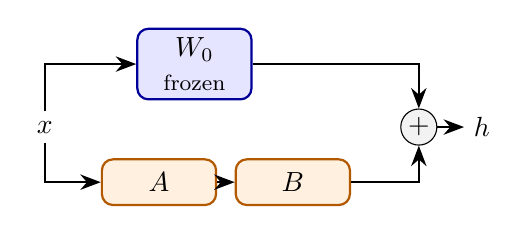
\begin{tikzpicture}[
                block/.style={
                    draw,
                    rounded corners=4pt,
                    minimum width=1.45cm,
                    minimum height=0.58cm,
                    align=center,
                    thick
                },
                frozen/.style={block, fill=blue!10, draw=blue!60!black},
                train/.style={block, fill=orange!12, draw=orange!70!black},
                arrow/.style={-{Stealth[length=2.6mm]}, thick}
            ]
                \node (x) at (0,0) {$x$};
                \node[frozen] (w0) at (1.9,0.8) {$W_0$ \\ \footnotesize frozen};
                \node[train] (a) at (1.45,-0.7) {$A$};
                \node[train] (b) at (3.15,-0.7) {$B$};
                \node[circle, draw, fill=gray!10, inner sep=1pt] (sum) at (4.75,0) {$+$};
                \node (h) at (5.55,0) {$h$};

                \draw[arrow] (x.north) |- (w0.west);
                \draw[arrow] (x.south) |- (a.west);
                \draw[arrow] (a.east) -- (b.west);
                \draw[arrow] (w0.east) -| (sum.north);
                \draw[arrow] (b.east) -| (sum.south);
                \draw[arrow] (sum.east) -- (h.west);
            \end{tikzpicture}
        \end{column}

        \begin{column}{0.44\textwidth}
            \textbf{Cơ chế cập nhật:}
            \[
                h = W_0x + \frac{\alpha}{r}BAx
            \]

            \textbf{Kích thước nhánh phụ:}
            \[
                A \in \mathbb{R}^{r \times d},
                \qquad
                B \in \mathbb{R}^{k \times r}
            \]

            \begin{block}{Tiết kiệm tham số}
                \[
                    \#\theta_{\mathrm{LoRA}}
                    =
                    r(d+k)
                    \ll
                    kd
                \]
                LoRA giả định rằng cập nhật khi fine-tune nằm trong một không gian con hạng thấp.
            \end{block}
        \end{column}
    \end{columns}
\end{frame}


% SLIDE 7: LoRTA & TensorGRAD
\begin{frame}{Mở rộng nâng cao: LoRTA và TensorGRAD}
    \textbf{\color{blue}LoRTA: tensor hóa cấu trúc cập nhật của LoRA}

    \[
        \Delta\mathcal{W}_{\ell,h,o,i}
        \approx
        \sum_{r=1}^{R}
        A_{\ell,r}
        B_{h,r}
        C_{o,r}
        D_{i,r}
    \]

    \begin{itemize}
        \item Gom các ma trận update đơn lẻ thành một tensor bậc cao.
        \item Khai thác cấu trúc adaptation giữa nhiều thành phần như \textit{layer} $(\ell)$, \textit{head} $(h)$, \textit{output} $(o)$ và \textit{input} $(i)$.
    \end{itemize}

    \vspace{0.25cm}

    \textbf{\color{blue}TensorGRAD: nén cấu trúc gradient động}

    \[
        \mathcal{G}_{\nabla}
        \approx
        \mathcal{C}
        \times_1 U^{(1)}
        \times_2
        \cdots
        \times_N U^{(N)}
    \]

    \begin{itemize}
        \item Dùng phân rã Tucker để xấp xỉ không gian gradient trong quá trình tối ưu.
        \item \textbf{Mục tiêu:} giảm bộ nhớ cần thiết khi lưu trữ gradient và trạng thái huấn luyện cho các toán tử mạng lớn.
    \end{itemize}
\end{frame}


% SLIDE 8: Poly-SA & Efficient Attention
\begin{frame}{Kiến trúc mới: Poly-SA và Attention hiệu quả}
    \begin{block}{Mô hình hóa chuỗi tuyến tính qua Hadamard Product}
        \[
            f_{\mathrm{Poly\mbox{-}SA}}(X)
            =
            \Psi\big((XW_1) \odot (XW_2)\big)
            \odot
            XW_3
        \]
    \end{block}

    \begin{itemize}
        \item \textbf{Cơ chế:} thay thế softmax attention tốn kém bằng chuỗi khai triển đa thức có cấu trúc.
        \item \textbf{Hiệu quả bộ nhớ:} giảm chi phí từ bậc hai $O(L^2)$ xuống gần tuyến tính theo độ dài chuỗi.
        \item \textbf{Thông điệp chính:} tensor product không chỉ dùng để nén mô hình, mà còn gợi ý cách thiết kế những khối kiến trúc mạng mới.
    \end{itemize}
\end{frame}


% SLIDE 10: Hạn chế
\begin{frame}{Hạn chế của phương pháp Tensor hóa}
    \begin{itemize}
        \item \textbf{Bài toán chọn rank:}
        rank quá thấp có thể làm mô hình thiếu năng lực biểu diễn và dẫn đến \textit{underfitting};
        rank quá cao lại làm mất lợi thế nén tham số.

        \item \textbf{Phụ thuộc vào ý nghĩa của mode:}
        các nhân tử sau phân rã chỉ dễ diễn giải khi các mode ban đầu có ý nghĩa rõ ràng, ví dụ như channel, head, layer hoặc token.

        \item \textbf{Chi phí tìm kiếm cấu trúc:}
        việc chọn CP, Tucker, TT hay vị trí tensor hóa trong mạng vẫn thường dựa nhiều vào thử nghiệm và kinh nghiệm.

        \item \textbf{Trade-off giữa hiệu quả và độ chính xác:}
        tensor hóa giúp giảm tham số và bộ nhớ, nhưng nếu chọn cấu trúc không phù hợp thì hiệu năng mô hình có thể suy giảm.
    \end{itemize}
\end{frame}


\section{Probabilistic Circuits}

\begin{frame}{Tensor xác suất và động lực}
\[
    \mathcal{P}\in
    \mathbb{R}^{|\mathcal{D}_1|\times\cdots\times|\mathcal{D}_N|},
    \qquad
    |\mathcal{P}|=\prod_{n=1}^{N}|\mathcal{D}_n|
\]
\begin{itemize}
    \item Mỗi entry là một xác suất $p(x_1,\ldots,x_N)$.
    \item Tensor xác suất đầy đủ tăng theo hàm mũ theo số biến.
    \item Tensor factorization biểu diễn gọn; circuit tổ chức phép tính để truy vấn hiệu quả.
\end{itemize}
\[
    \text{Tensor Factorization}
    \Longleftrightarrow
    \text{Circuit}
    \Longrightarrow
    \text{Tractable Inference}
\]
\end{frame}

\begin{frame}{Circuit là gì?}
\begin{columns}[T,totalwidth=\textwidth]
    \begin{column}{0.46\textwidth}
        \centering
        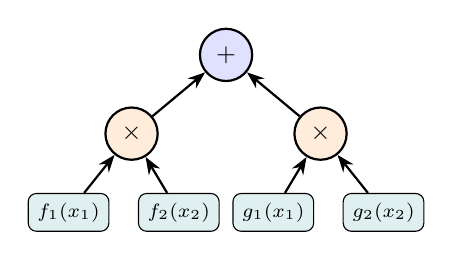
\begin{tikzpicture}[
            node/.style={circle, draw, thick, minimum size=0.62cm, font=\small},
            input/.style={rectangle, draw, rounded corners=3pt, fill=teal!12, minimum width=1.0cm, minimum height=0.45cm, font=\scriptsize},
            sum/.style={node, fill=blue!12},
            prod/.style={node, fill=orange!14},
            arrow/.style={-{Stealth[length=2.2mm]}, thick}
        ]
            \node[sum] (s) at (0,0) {$+$};
            \node[prod] (p1) at (-1.2,-1.0) {$\times$};
            \node[prod] (p2) at (1.2,-1.0) {$\times$};
            \node[input] (x1) at (-2.0,-2.0) {$f_1(x_1)$};
            \node[input] (x2) at (-0.6,-2.0) {$f_2(x_2)$};
            \node[input] (x3) at (0.6,-2.0) {$g_1(x_1)$};
            \node[input] (x4) at (2.0,-2.0) {$g_2(x_2)$};
            \draw[arrow] (x1) -- (p1);
            \draw[arrow] (x2) -- (p1);
            \draw[arrow] (x3) -- (p2);
            \draw[arrow] (x4) -- (p2);
            \draw[arrow] (p1) -- (s);
            \draw[arrow] (p2) -- (s);
        \end{tikzpicture}
    \end{column}
    \begin{column}{0.50\textwidth}
        \begin{itemize}
            \item Circuit là một DAG tham số hóa, tính hàm bằng forward pass theo thứ tự topo.
            \item Mỗi node có \textbf{scope}: tập biến mà node phụ thuộc.
            \item Kích thước $|c|$ thường tính bằng số node/cạnh/tham số.
        \end{itemize}
        \[
            c(x)=\sum_{j\in\mathrm{in}(n)}w_{n,j}c_j(x)
            \quad\text{hoặc}\quad
            c(x)=\prod_{j\in\mathrm{in}(n)}c_j(x)
        \]
    \end{column}
\end{columns}
\end{frame}

\begin{frame}{Circuit gồm những unit nào?}
\small
\begin{columns}[T,totalwidth=\textwidth]
    \begin{column}{0.32\textwidth}
        \textbf{Input unit}
        \[
            c_n(x_{S_n})=f_n(x_{S_n})
        \]
        \begin{itemize}
            \item Đọc biến hoặc hàm cục bộ.
            \item Scope nhỏ.
        \end{itemize}
    \end{column}
    \begin{column}{0.32\textwidth}
        \textbf{Product unit}
        \[
            c_n=\prod_{j\in\mathrm{in}(n)}c_j
        \]
        \begin{itemize}
            \item Ghép các scope con.
            \item Tractable khi decomposable.
        \end{itemize}
    \end{column}
    \begin{column}{0.32\textwidth}
        \textbf{Sum unit}
        \[
            c_n=\sum_{j\in\mathrm{in}(n)}w_{n,j}c_j
        \]
        \begin{itemize}
            \item Mixture/tổng có trọng số.
            \item Tractable khi smooth.
        \end{itemize}
    \end{column}
\end{columns}
\[
    \mathrm{scope}(n)=\bigcup_{j\in\mathrm{in}(n)}\mathrm{scope}(j)
\]
\end{frame}
\begin{frame}{CP decomposition như một circuit sum-product}
\begin{columns}[T,totalwidth=\textwidth]
    \begin{column}{0.60\textwidth}
        \centering
        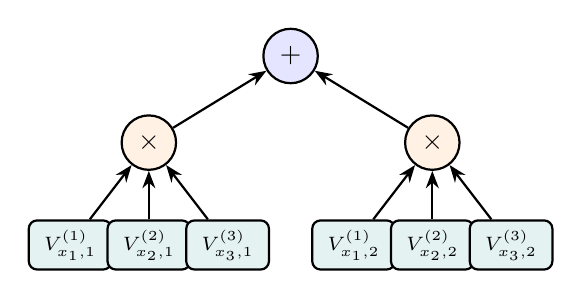
\begin{tikzpicture}[
            sum/.style={circle, draw, fill=blue!10, minimum size=0.65cm, thick},
            prod/.style={circle, draw, fill=orange!10, minimum size=0.65cm, thick},
            leaf/.style={rectangle, draw, rounded corners=3pt, fill=teal!10, minimum height=0.45cm, minimum width=1.05cm, thick, font=\scriptsize},
            arrow/.style={-{Stealth[length=2.2mm]}, thick}
        ]
            \node[sum] (out) at (0,0) {$+$};
            \node[prod] (p1) at (-1.8,-1.1) {$\times$};
            \node[prod] (p2) at (1.8,-1.1) {$\times$};
            \foreach \x/\name/\lab in {-2.8/l11/$V^{(1)}_{x_1,1}$,-1.8/l12/$V^{(2)}_{x_2,1}$,-0.8/l13/$V^{(3)}_{x_3,1}$} {
                \node[leaf] (\name) at (\x,-2.4) {\lab};
                \draw[arrow] (\name) -- (p1);
            }
            \foreach \x/\name/\lab in {0.8/l21/$V^{(1)}_{x_1,2}$,1.8/l22/$V^{(2)}_{x_2,2}$,2.8/l23/$V^{(3)}_{x_3,2}$} {
                \node[leaf] (\name) at (\x,-2.4) {\lab};
                \draw[arrow] (\name) -- (p2);
            }
            \draw[arrow] (p1) -- (out);
            \draw[arrow] (p2) -- (out);
        \end{tikzpicture}
    \end{column}
    \begin{column}{0.36\textwidth}
        \[
            \mathcal{T}_{x_1,x_2,x_3}
            =
            \sum_{r=1}^{R}
            V^{(1)}_{x_1,r}
            V^{(2)}_{x_2,r}
            V^{(3)}_{x_3,r}
        \]
        \begin{itemize}
            \item Product nodes: nhân theo mode.
            \item Sum node: cộng theo rank.
        \end{itemize}
    \end{column}
\end{columns}
\end{frame}

\begin{frame}{Tucker circuit và chi phí core}
\[
    \mathcal{T}_{x_1,\ldots,x_N}
    \approx
    \sum_{r_1,\ldots,r_N}
    \mathcal{W}_{r_1,\ldots,r_N}
    \prod_{n=1}^{N}V^{(n)}_{x_n,r_n}
\]
\begin{itemize}
    \item Tucker circuit dùng core tensor để trộn các latent dimensions.
    \item Kích thước circuit/core có thể tăng như:
    \[
        O\!\left(N\prod_{n=1}^{N}R_n\right)
    \]
    \item Khi core superdiagonal, Tucker trở về CP.
\end{itemize}
\end{frame}

\begin{frame}{Structural properties}
\small
\renewcommand{\arraystretch}{1.25}
\begin{tabular}{p{0.24\textwidth}p{0.38\textwidth}p{0.28\textwidth}}
\toprule
\textbf{Property} & \textbf{Điều kiện} & \textbf{Cho phép} \\
\midrule
Smoothness & Các nhánh vào sum node có cùng scope & Marginalization đúng \\
Decomposability & Các nhánh vào product node có scope rời nhau & Tách tích phân theo nhóm biến \\
Compatibility & Hai circuits chia scope cùng cấu trúc & Tính expectation giữa $p$ và $f$ \\
Determinism & Supports của nhánh sum rời nhau & MAP inference hiệu quả hơn \\
\bottomrule
\end{tabular}
\[
    \text{smooth + decomposable}
    \Rightarrow
    \text{marginals trong }O(|c|)
\]
\end{frame}

\begin{frame}{Truy vấn suy luận: marginal và conditional}
\begin{columns}[T,totalwidth=\textwidth]
    \begin{column}{0.48\textwidth}
        \textbf{Marginal}
        \[
            p(\mathbf{x}_O)
            =
            \sum_{\mathbf{x}_M\in\mathcal{D}_M}
            p(\mathbf{x}_O,\mathbf{x}_M)
        \]
        \begin{itemize}
            \item $O$: biến quan sát, $M$: biến bị sum-out.
            \item Smooth + decomposable $\Rightarrow O(|c|)$.
        \end{itemize}
    \end{column}
    \begin{column}{0.48\textwidth}
        \textbf{Conditional}
        \[
            p(\mathbf{x}_M\mid\mathbf{x}_O)
            =
            \frac{p(\mathbf{x}_O,\mathbf{x}_M)}
            {\sum_{\mathbf{x}'_M}p(\mathbf{x}_O,\mathbf{x}'_M)}
        \]
        \begin{itemize}
            \item Tử số: evaluate circuit tại assignment.
            \item Mẫu số: marginalize biến missing.
        \end{itemize}
    \end{column}
\end{columns}
\end{frame}

\begin{frame}{Truy vấn suy luận dưới góc nhìn tensor factorization}
\[
    c(x_1,\ldots,x_N)
    =
    \sum_{r=1}^{R}\prod_{n=1}^{N}V^{(n)}_{x_n,r}
\]
\[
    c(\mathbf{x}_O)
    =
    \sum_{r=1}^{R}
    \left(\prod_{n\in O}V^{(n)}_{x_n,r}\right)
    \left(\prod_{m\in M}\sum_{x_m\in\mathcal{D}_m}V^{(m)}_{x_m,r}\right)
\]
\begin{itemize}
    \item Marginalize một mode $m$ bằng cách thay factor $V^{(m)}_{x_m,r}$ bởi tổng theo hàng của mode đó.
    \item Vì product node decomposable, phép cộng trên nhiều assignment được đẩy xuống từng factor matrix.
\end{itemize}
\end{frame}

\begin{frame}{Truy vấn suy luận: expectation}
\[
    \mathbb{E}_{\mathbf{x}\sim p}[f(\mathbf{x})]
    =
    \sum_{\mathbf{x}}p(\mathbf{x})f(\mathbf{x})
    =
    \langle\mathcal{P},\mathcal{F}\rangle
\]
\begin{itemize}
    \item Nếu $p$ và $f$ là hai circuits compatible, có thể tính bằng product circuit rồi marginalize.
    \item Dưới góc nhìn TF: contract tensor xác suất $\mathcal{P}$ với tensor hàm $\mathcal{F}$.
    \item Ứng dụng trong report: missing values, fairness query, adversarial robustness.
\end{itemize}
\[
    \mathbb{E}[f(\mathbf{x})\mid A=0]-\mathbb{E}[f(\mathbf{x})\mid A=1]
\]
\end{frame}

\begin{frame}{Truy vấn suy luận: MAP và sampling}
\begin{columns}[T,totalwidth=\textwidth]
    \begin{column}{0.48\textwidth}
        \textbf{MAP / MPE}
        \[
            \mathbf{x}^{\star}
            =
            \arg\max_{\mathbf{x}}p(\mathbf{x}\mid\mathbf{e})
        \]
        \begin{itemize}
            \item Cần thêm determinism để tối ưu tractable hơn.
            \item Sum node chọn nhánh tốt nhất thay vì cộng tất cả nhánh.
        \end{itemize}
    \end{column}
    \begin{column}{0.48\textwidth}
        \textbf{Sampling top-down}
        \begin{itemize}
            \item Sum node: lấy mẫu nhánh categorical theo trọng số.
            \item Product node: đi qua tất cả nhánh con vì scope rời nhau.
            \item Leaf/input: lấy mẫu biến quan sát cục bộ.
        \end{itemize}
    \end{column}
\end{columns}
\end{frame}
\begin{frame}{Non-negative TF như latent variable model}
\[
    p(x)
    =
    \sum_{r=1}^{R}p(r)\prod_{n=1}^{N}p_n(x_n\mid r)
\]
\begin{itemize}
    \item Chỉ số rank $r$ có thể đọc như latent component.
    \item Sum node tương ứng với mixture variable.
    \item Product node sinh độc lập trên các scope rời nhau.
    \item Sampling thực hiện top-down: chọn nhánh ở sum, đi qua tất cả nhánh ở product.
\end{itemize}
\end{frame}

\begin{frame}{Demo CPJ Circuit}
\centering
\renewcommand{\arraystretch}{1.25}
\begin{tabular}{p{0.28\textwidth}p{0.30\textwidth}p{0.30\textwidth}}
\toprule
\textbf{Demo} & \textbf{Thiết lập} & \textbf{Kết quả chính} \\
\midrule
Toy 4-bit & $2^4=16$ assignments & KL(target $\Vert$ circuit) $=0.0054$; tổng xác suất $=1.000000$ \\
Binarized MNIST & $28\times 28=784$ biến nhị phân & Best val bpd $=0.3675$; test bpd $=0.3704$ \\
\bottomrule
\end{tabular}
\[
    \mathrm{bpd}=-\frac{\log p(x)}{784\log 2}
\]
\end{frame}

\begin{frame}{Hạn chế và câu hỏi mở của PC}
\begin{itemize}
    \item Tractable inference không đảm bảo biểu diễn luôn nhỏ.
    \item Tucker/core có thể tăng theo $R^N$ nếu số mode lớn.
    \item Hiệu quả phụ thuộc region graph, width/rank và cấu trúc phụ thuộc thật trong dữ liệu.
    \item Câu hỏi mở: optimization, identifiability, approximate inference, scalability.
\end{itemize}
\end{frame}

\section{Interpretable Data Mining}

\begin{frame}{Vì sao CP hữu ích cho data mining?}
\large
\begin{itemize}
    \item Dữ liệu khoa học thường có các mode như subject, time, metabolite, electrode/voxel.
    \item CP giữ các mode riêng thay vì trải phẳng thành ma trận.
    \item Mỗi component có thể được đọc như một pattern đồng thời trên nhiều trục.
\end{itemize}
\[
    \mathcal{X}\approx\cp{\mathbf{A}^{(1)},\ldots,\mathbf{A}^{(N)}}.
\]
\end{frame}

\begin{frame}{CP-ALS}
\large
\[
    \mathbf{Z}^{(n)}
    =
    \mathbf{A}^{(N)}\odot\cdots\odot\mathbf{A}^{(n+1)}
    \odot\mathbf{A}^{(n-1)}\odot\cdots\odot\mathbf{A}^{(1)}.
\]
\[
    \mathbf{A}^{(n)}
    \leftarrow
    \underbrace{\mathbf{X}_{(n)}\mathbf{Z}^{(n)}}_{\text{MTTKRP}}
    \left((\mathbf{Z}^{(n)})^\top\mathbf{Z}^{(n)}\right)^\dagger.
\]
\begin{itemize}
    \item Lặp qua từng mode, cố định các factor còn lại.
    \item Bottleneck tính toán là MTTKRP.
\end{itemize}
\end{frame}

\begin{frame}{CP-OPT, missing data và loss khác}
\large
\begin{itemize}
    \item CP-OPT tối ưu tất cả factor matrices cùng lúc bằng gradient-based optimizer.
    \item CP-WOPT dùng weight tensor để chỉ fit trên entries quan sát:
    \[
        \min\left\|
        \mathcal{W}\had(\mathcal{X}-\cp{\mathbf{A}^{(1)},\ldots,\mathbf{A}^{(N)}})
        \right\|_F^2.
    \]
    \item GCP-OPT thay Frobenius loss bằng loss phù hợp với count/binary data.
\end{itemize}
\end{frame}

\begin{frame}{PARAFAC2}
\large
\[
    \mathbf{X}_k\approx \mathbf{U}_k\mathbf{S}_k\mathbf{V}^{\top},
    \qquad
    \mathbf{U}_k^\top\mathbf{U}_k=\boldsymbol{\Phi}.
\]
\begin{itemize}
    \item Nới lỏng strict multilinearity của CP.
    \item Cho phép một factor thay đổi theo slice.
    \item Phù hợp dữ liệu time-evolving hoặc các chuỗi có độ dài/căn pha khác nhau.
\end{itemize}
\end{frame}

\begin{frame}{CMTF và data fusion}
\large
\[
    \min_{\mathbf{A},\mathbf{B},\mathbf{C},\mathbf{D}}
    \|\mathcal{X}-\cp{\mathbf{A},\mathbf{B},\mathbf{C}}\|_F^2
    +
    \|\mathbf{Y}-\mathbf{A}\mathbf{D}^{\top}\|_F^2.
\]
\begin{itemize}
    \item Joint analysis cho nhiều matrix/tensor có mode chung.
    \item Factor $\mathbf{A}$ liên kết hai nguồn dữ liệu theo subject.
    \item Coupling có thể cải thiện uniqueness và chất lượng pattern discovery.
\end{itemize}
\end{frame}

\begin{frame}{Ứng dụng trong tutorial}
\large
\begin{itemize}
    \item \textbf{Metabolomics}: tìm marker và pattern phản ứng chuyển hóa.
    \item \textbf{Neuroscience}: phân tích EEG/fMRI theo không gian, thời gian, subject.
    \item \textbf{Gut microbiome}: rút trích pattern cộng đồng vi sinh theo thời gian.
    \item \textbf{Data fusion}: kết hợp dữ liệu động và tĩnh trên cùng nhóm subject.
\end{itemize}
\end{frame}

\section{Thực nghiệm}

\begin{frame}{Tổng quan các demo}
\centering
\small
\renewcommand{\arraystretch}{1.3}
\begin{tabular}{>{\raggedright\arraybackslash}p{0.22\textwidth}>{\raggedright\arraybackslash}p{0.34\textwidth}>{\raggedright\arraybackslash}p{0.31\textwidth}}
\toprule
\textbf{Demo} & \textbf{Mục tiêu} & \textbf{Metric chính} \\
\midrule
LoRA rank sweep & Kiểm tra parameter-efficient adaptation & accuracy, trainable params, loss \\
CPJ Circuit & Kiểm tra tensor xác suất và tractable density estimation & KL, log-likelihood, bpd \\
Data Mining & Kiểm tra khả năng giữ cấu trúc đa mode & FMS, fit score, shared factor \\
\bottomrule
\end{tabular}
\end{frame}

\begin{frame}{LoRA rank sweep: thiết lập}
\begin{columns}[T,totalwidth=\textwidth]
    \begin{column}{0.48\textwidth}
        \begin{itemize}
            \item Dataset: GLUE SST-2 sentiment classification.
            \item Model: \texttt{prajjwal1/bert-tiny}.
            \item Train subset: 5000 mẫu; validation: 872 mẫu.
            \item Mỗi cấu hình chạy 3 epochs, seed 42.
        \end{itemize}
    \end{column}
    \begin{column}{0.48\textwidth}
        \small
        \renewcommand{\arraystretch}{1.1}
        \begin{tabular}{ll}
        \toprule
        \textbf{Config} & \textbf{Chế độ} \\
        \midrule
        frozen & freeze encoder \\
        full fine-tune & cập nhật toàn bộ model \\
        LoRA r=2 & rank thấp \\
        LoRA r=4 & rank trung bình \\
        LoRA r=8 & rank cao hơn \\
        \bottomrule
        \end{tabular}
    \end{column}
\end{columns}
\end{frame}

\begin{frame}{LoRA rank sweep: kết quả}
\begin{columns}[T,totalwidth=\textwidth]
    \begin{column}{0.58\textwidth}
        \centering
        
\includegraphics[width=\linewidth]{accuracy_vs_params.png}
    \end{column}
    \begin{column}{0.38\textwidth}
        \small
        \renewcommand{\arraystretch}{1.15}
        \begin{tabular}{lcc}
        \toprule
        \textbf{Config} & \textbf{Params} & \textbf{Acc} \\
        \midrule
        Frozen & 258 & 0.6525 \\
        Full & 4,386,178 & 0.7569 \\
        LoRA r=2 & 2,306 & 0.7248 \\
        LoRA r=4 & 4,354 & 0.7351 \\
        LoRA r=8 & 8,450 & \textbf{0.7511} \\
        \bottomrule
        \end{tabular}
    \end{column}
\end{columns}
\end{frame}

\begin{frame}{LoRA rank sweep: nhận xét}
\begin{itemize}
    \item LoRA rank 8 chỉ kém full fine-tuning khoảng $0.57$ điểm accuracy.
    \item Số tham số trainable giảm từ $4{,}386{,}178$ xuống $8{,}450$.
    \item Best accuracy tăng khi rank tăng từ 2 lên 8 trong lần chạy này.
    \item Kết quả không nên xem là benchmark đầy đủ: model nhỏ, subset nhỏ, chỉ 3 epochs.
\end{itemize}
\[
    \text{LoRA r=8: }0.1923\%\text{ tham số trainable}
    \quad\text{và}\quad
    \approx 519\times\text{ ít tham số hơn full fine-tune}
\]
\end{frame}

\begin{frame}{CPJ Circuit: toy 4-bit -- hội tụ}
\begin{columns}[T,totalwidth=\textwidth]
    \begin{column}{0.45\textwidth}
        \begin{itemize}
            \item Target distribution trên 4 biến nhị phân: $2^4=16$ tensor entries.
            \item Target có tương quan \texttt{same-pair}, \texttt{xor-pair} và parity.
            \item Train set: 2000 mẫu sinh từ target distribution.
            \item Binary CPJ Circuit, width $K=8$, Adam, 300 epochs.
        \end{itemize}
    \end{column}
    \begin{column}{0.51\textwidth}
        \centering
        \small
        \renewcommand{\arraystretch}{1.18}
        \begin{tabular}{rcc}
        \toprule
        \textbf{Epoch} & \textbf{Train NLL} & \textbf{KL}$(p^*\Vert p_\theta)$ \\
        \midrule
        1   & 2.7727 & 0.2967 \\
        100 & 2.6111 & 0.1281 \\
        200 & 2.5225 & 0.0360 \\
        300 & \textbf{2.5000} & \textbf{0.0054} \\
        \bottomrule
        \end{tabular}

        \vspace{0.12cm}
        \[
            \sum_{\mathbf{x}}p_\theta(\mathbf{x})=1.000000
        \]
    \end{column}
\end{columns}
\end{frame}

\begin{frame}{CPJ Circuit: enumerate tensor xác suất}
\centering
\small
\renewcommand{\arraystretch}{1.18}
\begin{tabular}{ccc}
\toprule
\textbf{Assignment} & \textbf{Target $p^*(\mathbf{x})$} & \textbf{Circuit $p_\theta(\mathbf{x})$} \\
\midrule
0000 & 0.07009 & 0.07131 \\
0001 & 0.12772 & 0.13048 \\
0111 & 0.00521 & 0.00739 \\
1000 & 0.00521 & 0.00479 \\
1101 & 0.12772 & 0.13111 \\
1111 & 0.07009 & 0.07751 \\
\bottomrule
\end{tabular}

\vspace{0.35cm}
\begin{itemize}
    \item Enumerate toàn bộ 16 assignments để kiểm tra trực tiếp tensor xác suất.
    \item KL giảm từ $0.2967$ xuống $0.0054$: circuit khớp gần sát target.
    \item Tổng xác suất bằng $1.000000$: CPJ định nghĩa phân phối chuẩn hóa.
\end{itemize}
\end{frame}

\begin{frame}{CPJ Circuit: Binarized MNIST -- thiết lập}
\begin{columns}[T,totalwidth=\textwidth]
    \begin{column}{0.50\textwidth}
        \begin{itemize}
            \item Ảnh $28\times28$ threshold tại 0.5.
            \item Mỗi ảnh thành vector 784 biến nhị phân.
            \item Tensor xác suất đầy đủ có $2^{784}$ entries, không thể materialize.
            \item Mục tiêu: density estimation, không phải classification.
        \end{itemize}
    \end{column}
    \begin{column}{0.46\textwidth}
        \small
        \renewcommand{\arraystretch}{1.18}
        \begin{tabular}{ll}
        \toprule
        \textbf{Hyperparameter} & \textbf{Giá trị} \\
        \midrule
        Train / Val / Test & 1000 / 200 / 200 \\
        Width $K$ & 8 \\
        Epochs & 50 \\
        Batch size & 128 \\
        Optimizer & Adam \\
        Learning rate & $10^{-2}$ \\
        Device & CUDA \\
        \bottomrule
        \end{tabular}
    \end{column}
\end{columns}
\end{frame}

\begin{frame}{CPJ Circuit: Binarized MNIST -- kết quả}
\centering
\small
\renewcommand{\arraystretch}{1.15}
\begin{tabular}{rcccc}
\toprule
\textbf{Epoch} & \textbf{Train NLL} & \textbf{Val LL} & \textbf{Val bpd} & \textbf{Time} \\
\midrule
1  & 524.178 & -499.040 & 0.9183 & 5.0s \\
10 & 294.150 & -284.672 & 0.5238 & 4.3s \\
20 & 231.515 & -226.047 & 0.4160 & 4.4s \\
30 & 213.894 & -208.713 & 0.3841 & 4.3s \\
40 & 207.032 & -201.993 & 0.3717 & 4.3s \\
50 & \textbf{204.571} & \textbf{-199.710} & \textbf{0.3675} & 4.4s \\
\bottomrule
\end{tabular}

\vspace{0.12cm}
\[
    \text{Best val LL}=-199.710,\quad
    \text{Test LL}=-201.305,\quad
    \text{Test bpd}=0.3704.
\]
\end{frame}

\begin{frame}{CPJ Circuit: nhận xét từ số liệu}
\begin{itemize}
    \item Toy 4-bit kiểm tra đúng tính chất cốt lõi: CPJ tính từng entry $p(\mathbf{x})$ của tensor xác suất và vẫn chuẩn hóa.
    \item KL $0.0054$ cho thấy width $K=8$ đủ khớp các tương quan nhỏ trong target distribution.
    \item MNIST scale số biến từ 4 lên 784 mà không dựng tensor $2^{784}$.
    \item Validation bpd giảm từ $0.9183$ xuống $0.3675$; test bpd $0.3704$.
    \item Đây là demo pipeline quy mô nhỏ, không phải benchmark cuối cùng: subset 1000 train và width $K=8$.
\end{itemize}
\end{frame}

\begin{frame}{Kết quả Data Mining}
\begin{columns}[T,totalwidth=\textwidth]
    \begin{column}{0.45\textwidth}
        \centering
        \small
        \renewcommand{\arraystretch}{1.12}
        \begin{tabular}{@{}lcc@{}}
        \toprule
        \textbf{Noise} & \textbf{CP-ALS} & \textbf{CP-OPT} \\
        \midrule
        $0.1$ & $\approx 1.00$ & $\approx 0.75$ \\
        $1$ & high & medium \\
        $>10$ & drops & drops \\
        \bottomrule
        \end{tabular}

        \vspace{0.12cm}
        \scriptsize FMS trend from the synthetic CP experiment.

        \vspace{0.1cm}
        CP-ALS giữ FMS gần $1.0$ khi noise nhỏ ($noise = 0.1$); FMS giảm rõ khi noise rất lớn ($noise > 10$). \\
        CP-OPT giữ FMS ở mức $0.75$ khi noise nhỏ ($noise = 0.1$); FMS giảm rõ khi noise rất lớn ($noise > 10$).
    \end{column}
    \begin{column}{0.51\textwidth}
        \small
        \renewcommand{\arraystretch}{1.15}
        \begin{tabular}{lcc}
        \toprule
        \textbf{Demo} & \textbf{Chỉ số} & \textbf{Kết quả} \\
        \midrule
        CP-ALS & FMS & \textbf{0.9999} \\
        CP-OPT & FMS & 0.7433 \\
        PARAFAC2 & Hội tụ & 5 vòng \\
        CMTF & Corr$(A,y)$ & 0.9971 \\
        \bottomrule
        \end{tabular}

        \vspace{0.05cm}
        \begin{itemize}\setlength\itemsep{0.1em}
            \item Thông số: Synthetic tensor =  $10\times15\times20$, truerank $3$, noise $=0.1$.
            \item EEG dạng tensor: $20\times64\times481$ giữ subject/channel/time.
            \item Rank EEG chọn tự động: $R=2$ với CORCONDIA $89.1\%$.
            \item SVD/PCA phải unfold thành $20\times30784$, làm trộn channel và time.
        \end{itemize}
    \end{column}
\end{columns}
\end{frame}

\begin{frame}{Data Mining: CP-ALS vs CP-OPT}
\centering
\renewcommand{\arraystretch}{1.25}
\begin{tabular}{lccc}
\toprule
\textbf{Thuật toán} & \textbf{Vòng lặp} & \textbf{Sai số tái tạo} & \textbf{FMS} \\
\midrule
CP-ALS & 5 & \textbf{0.0601} & \textbf{0.9999} \\
CP-OPT (L-BFGS-B) & 9 & 0.2195 & 0.7433 \\
\bottomrule
\end{tabular}

\vspace{0.35cm}
\begin{itemize}
    \item Tensor synthetic kích thước $10\times15\times20$, noise $=0.1$.
    \item TrueRank $R=3$; CP-ALS khôi phục factor gần như trùng ground truth.
    \item Không kết luận CP-ALS luôn tốt hơn CP-OPT; CP-OPT linh hoạt hơn với loss/ràng buộc khác.
\end{itemize}
\end{frame}

\begin{frame}{Data Mining: PARAFAC2 và CMTF}
\begin{columns}[T,totalwidth=\textwidth]
    \begin{column}{0.48\textwidth}
        \textbf{PARAFAC2}
        \begin{itemize}
            \item $K=5$ subjects, slice sizes $[87,87,87,87,87]\times64$.
            \item Rank $R=2$.
            \item Hội tụ sau 5 vòng; $V$ có shape $64\times2$.
        \end{itemize}
    \end{column}
    \begin{column}{0.48\textwidth}
        \textbf{CMTF}
        \begin{itemize}
            \item Tensor EEG: $20\times64\times481$.
            \item Metadata giả lập: $20\times5$.
            \item Hội tụ: 10 vòng với $Y$, 20 vòng với $Y_{\text{null}}$.
            \item Sai số tái thiết: $X=576.6580$, $Y=2702.3291$.
            \item Corr tốt nhất giữa $A$ và nhãn chẵn/lẻ: $0.9971$ ở component 1.
        \end{itemize}
    \end{column}
\end{columns}
\[
    \min \|\mathcal{X}-\cp{A,B,C}\|_F^2+\|Y-AD^\top\|_F^2
\]
\end{frame}

\begin{frame}{Data Mining: SVD/PCA vs CP-ALS trên EEG}
\begin{columns}[T,totalwidth=\textwidth]
    \begin{column}{0.48\textwidth}
        \centering
        
\includegraphics[width=\linewidth]{DM_02_0.png}
        \vspace{0.1cm}
    \end{column}
    \begin{column}{0.48\textwidth}
        \small
        \renewcommand{\arraystretch}{1.2}
        \begin{tabular}{@{}ll@{}}
        \toprule
        \textbf{Method} & \textbf{Summary} \\
        \midrule
        SVD/PCA & Unfolds to $20\times30784$. \\
        CP-ALS & Keeps $20\times64\times481$. \\
        \bottomrule
        \end{tabular}

        \vspace{0.25cm}
        \begin{itemize}\setlength\itemsep{0.05em}
            \item CP-ALS chọn $R=2$ với fit cuối $0.08936$.
            \item CORCONDIA đạt $89.1\%$ tại $R=2$.
            \item Rank lớn hơn giảm error nhưng CORCONDIA âm mạnh.
        \end{itemize}
        \scriptsize $R=2$ cân bằng tốt giữa fit và ổn định cấu trúc.
    \end{column}
\end{columns}
\end{frame}



\begin{frame}{Kết luận}
\large
\begin{itemize}
    \item Tensor factorization giúp biến dữ liệu nhiều chiều thành cấu trúc có thể nén và diễn giải.
    \item CP/Tucker là nền tảng chung cho LoRA, probabilistic circuits và khai phá dữ liệu đa mode.
    \item Các demo cho thấy cùng một ý tưởng low-rank xuất hiện ở cả tham số mô hình, tensor xác suất và dữ liệu EEG.
\end{itemize}
\end{frame}

\begin{frame}
    \centering
    \Huge Cảm ơn thầy và các bạn
\end{frame}

\end{document}
